\documentclass[12pt]{article}

\title{Using language as an indicator of cognitive decline in pre-clinical Alzheimer's Disease.}

\author{
	Jomar Alcantara \\
	Department of Computer Science\\
	School of Engineering and Applied Sciences\\
	Aston University\\
	\texttt{alcantaj@aston.ac.uk} \\
		\and
	\textbf{Peter Sawyer} \\
	Department of Computer Science\\
	School of Engineering and Applied Sciences\\
	Aston University\\
	\texttt{p.sawyer@aston.ac.uk} \\
		\and
	George Vogiatzis\\
	Department of Computer Science\\
	School of Engineering and Applied Sciences\\
	Aston University \\
	\texttt{g.vogiatzis@aston.ac.uk} \\
		\and
	\textbf{Felipe Campelo}\\
	Department of Computer Science\\
	School of Engineering and Applied Sciences\\
	Aston University\\
	\texttt{f.campelo@aston.ac.uk}
}
\date{\today}

\usepackage{float}
\usepackage{graphicx}
\usepackage{color}

\begin{document}

\bigskip
\begin{abstract}
Several research efforts aimed at improving the early diagnosis of Alzheimer's Disease have focused on the longitudinal analysis of lexical features which have been implicated in the pre-clinical progression of this disease. We build on these studies to develop a refined method for extracting and analysing language from transcripts. Our method is based on a statistical evaluation of the most relevant features, as well as on the use of Generalised Additive Models instead of Linear Regression as a way to more adequately model the declines in language over time. We evaluate our method using the unscripted question and answer portions of news conferences from three U.S Presidents: Ronald Reagan (RR), who would later go on to receive a diagnosis of Alzheimer's Disease; George H. W. Bush (GB) and Donald Trump (DT), who have no known diagnosis of dementia. Our controls were the closest in age to RR when they became president. Our analysis uncovered several lexical features that did not change significantly for GB and DT, but presented significant changes for RR. These included decreases in unique words and noun usage, and significant increases in pronouns and conjunctions and also words which are related to social processes significantly increase over time. We also show that non-linear models provide a more detailed way to model these changes over time that is sensitive to variability in the degrees of change that is typical of AD. Our findings are consistent with the psychological literature, which documents a link between these features and cognitive decline in Alzheimer's Disease. This work demonstrates that there are potentially a wider number of language markers that researchers can track, which may indicate the presence of mild cognitive impairment as well as illustrating a more nuanced way of modelling these changes via Generalised Additive Models.
\end{abstract}

\maketitle
\section{Introduction}\label{introduction}
A diagnosis of dementia is generally made when there is a decline in brain function due to physical changes in the brain \cite{Albert2011}. It affects a significant proportion of the global older adult population and the impact on morbidity and mortality rates is considerable. Dementia including Alzheimer's Disease is currently the leading cause of death in England and Wales \cite{Patel2018} and the sixth leading cause of death in the United States (US) accounting for 32\% of all adult deaths in the US and projected to rise to 43\% by 2050 \cite{Weuve2014} . A 2014 report commissioned by the Alzheimer's Society estimated that in the UK by 2015 there would be approximately 855,000 people rising living with dementia increasing to 1 million by 2021 \cite{AlzheimersSociety2014}. This represents 1 in 79 of the total UK population rising to 1 in 14 of those aged 65 or over \cite{AlzheimersSociety2014}. Worldwide, there are 46 million people with a diagnosis of dementia globally and that number is expected to hit 131.5 million by 2050 \cite{Prince2015}. From a financial perspective, the cost burden is also significant. The estimated annual spend on dementia healthcare in the UK is £4.3 billion of which approximately £85 million is spent on diagnosis. The total financial burden of dementia (excluding the costs associated with early onset dementia) is £26.3 billion annually. Globally, this picture is a lot bleaker. The worldwide cost of dementia in 2018 was estimated to be in the region of one trillon US dollars \cite{Prince2015}.
\par 
There are different types of dementia including Alzheimer's Disease (AD), vascular dementia, dementia with Lewy bodies and fronto-temporal dementia, all of which are currently incurable. AD is a progressive neurodegenerative disease and is the most common type of dementia, responsible for approximately 60\% to 80\% of all cases \cite{Duong2017}. Currently, a definitive diagnosis for AD can only be produced post-mortem. However, there are a number of psychological and physiological indicators that can indicate that AD is is present. These physiological changes lead to the development of some of the psychological symptoms associated with AD, primarily cognitive deficits such as problems with episodic and semantic memory, organizing and planning and other problems with executive function, difficulties with language, and visuospatial deficits \cite{McKhann2011}. These cognitive symptoms are often accompanied by emotional problems such as depression and behavioural difficulties. As more neurons die throughout the brain, a person with AD gradually loses the ability to think, remember, make decisions and function independently.
\par
Despite the increasing prevalence of AD and an improved understanding about how it affects the brain there are no medications that improve prognosis. All the medications that are currently on the market are designed to manage symptoms. Whilst there are numerous investigational drugs in development for the treatment of AD, a larger than normal percentage of these drugs fail in the clinical trial stage of the drug discovery process (99.6\% failure rate vs 80\% for systemic anti-cancer drugs) \cite{Cummings2014}. Cummings et al proposed that a possible reason for the lack of success is that the drug treatments are initiated too far along in the progression of the disease and thus much of the degeneration of the brain has already occurred \cite{Cummings2014}. Research focus has now started to shift to the earlier stages of AD (i.e. symptomatic pre-dementia phase of AD) which some literature describes as 'Mild Cognitive Impairment (MCI) due to AD'.
\par
One of the challenges associated with the early detection of AD is differentiating natural age associated memory impairment and cognitive decline due to aging from decline due to AD \cite{Lo2017}. This challenge is often complicated further due to the large variation in the cognitive abilities and educational background of individuals \cite{Harada2013}. The work of Albert et al helps to address this by the development of clinical criteria which professionals can use to diagnose MCI due to AD. One of the most important observations from this piece of work is that a diagnosis of MCI requires evidence of intra-individual change and optimally requires evaluation at two or more points \cite{Albert2011}.This is essentially to place more importance on the trajectory of a person's cognitive abilities rather than a person's cognitive ability in general. Berisha and Liss used the transcripts of press conferences of Ronald Reagan who would go on to be diagnosed with AD, and George Bush Sr who had no diagnosis. These speeches are in the public domain and provide a good opportunity of analysing the spontaneous language use of someone with AD, before a diagnosis was made. 
\par 
There has been significant research in the area of language deterioration as a method of detecting AD at an earlier stage. This usually takes the form of recording speech whilst patients' undertake a cognitive assessment such as the Picture Description Task \cite{Fraser2015}. Given that language samples are relatively easy to collect, research has moved towards analysis of spontaneous speech. The work of Berisha and Liss is a good example of this, their study compared the differences in language use between two US presidents, Ronald Reagan (RR), who would go on to receive a diagnosis of Dementia and George H. W. Bush (GHWB) who acted as a matched control based on Age \cite{Berisha2015}. They found several differences in language use over time which they felt acted as indicators of RR's difficulties with language due to AD. Differences in features of language identified to be statistically significant included the number of unique words used per speech, the use of non-specific nouns and fillers and low imageability verbs \cite{Berisha2015}. 
\par
% Stronger motivation
Berisha and Liss have developed interesting ideas about how we might track changes over time in various lexical features which have been associated with the development of Alzheimer's Disease. However we feel that cognitive decline in pre-clinical AD is not accurately modeled as a linear process and therefore we explored the application of generalised additive models (GAMs) to this data which have no assumed understanding of the distribution of the data. We refine these ideas with the aim of exploring the potential for a protocol that can be used for analyzing language deterioration. 

\begin{figure}[H]
	\centering
	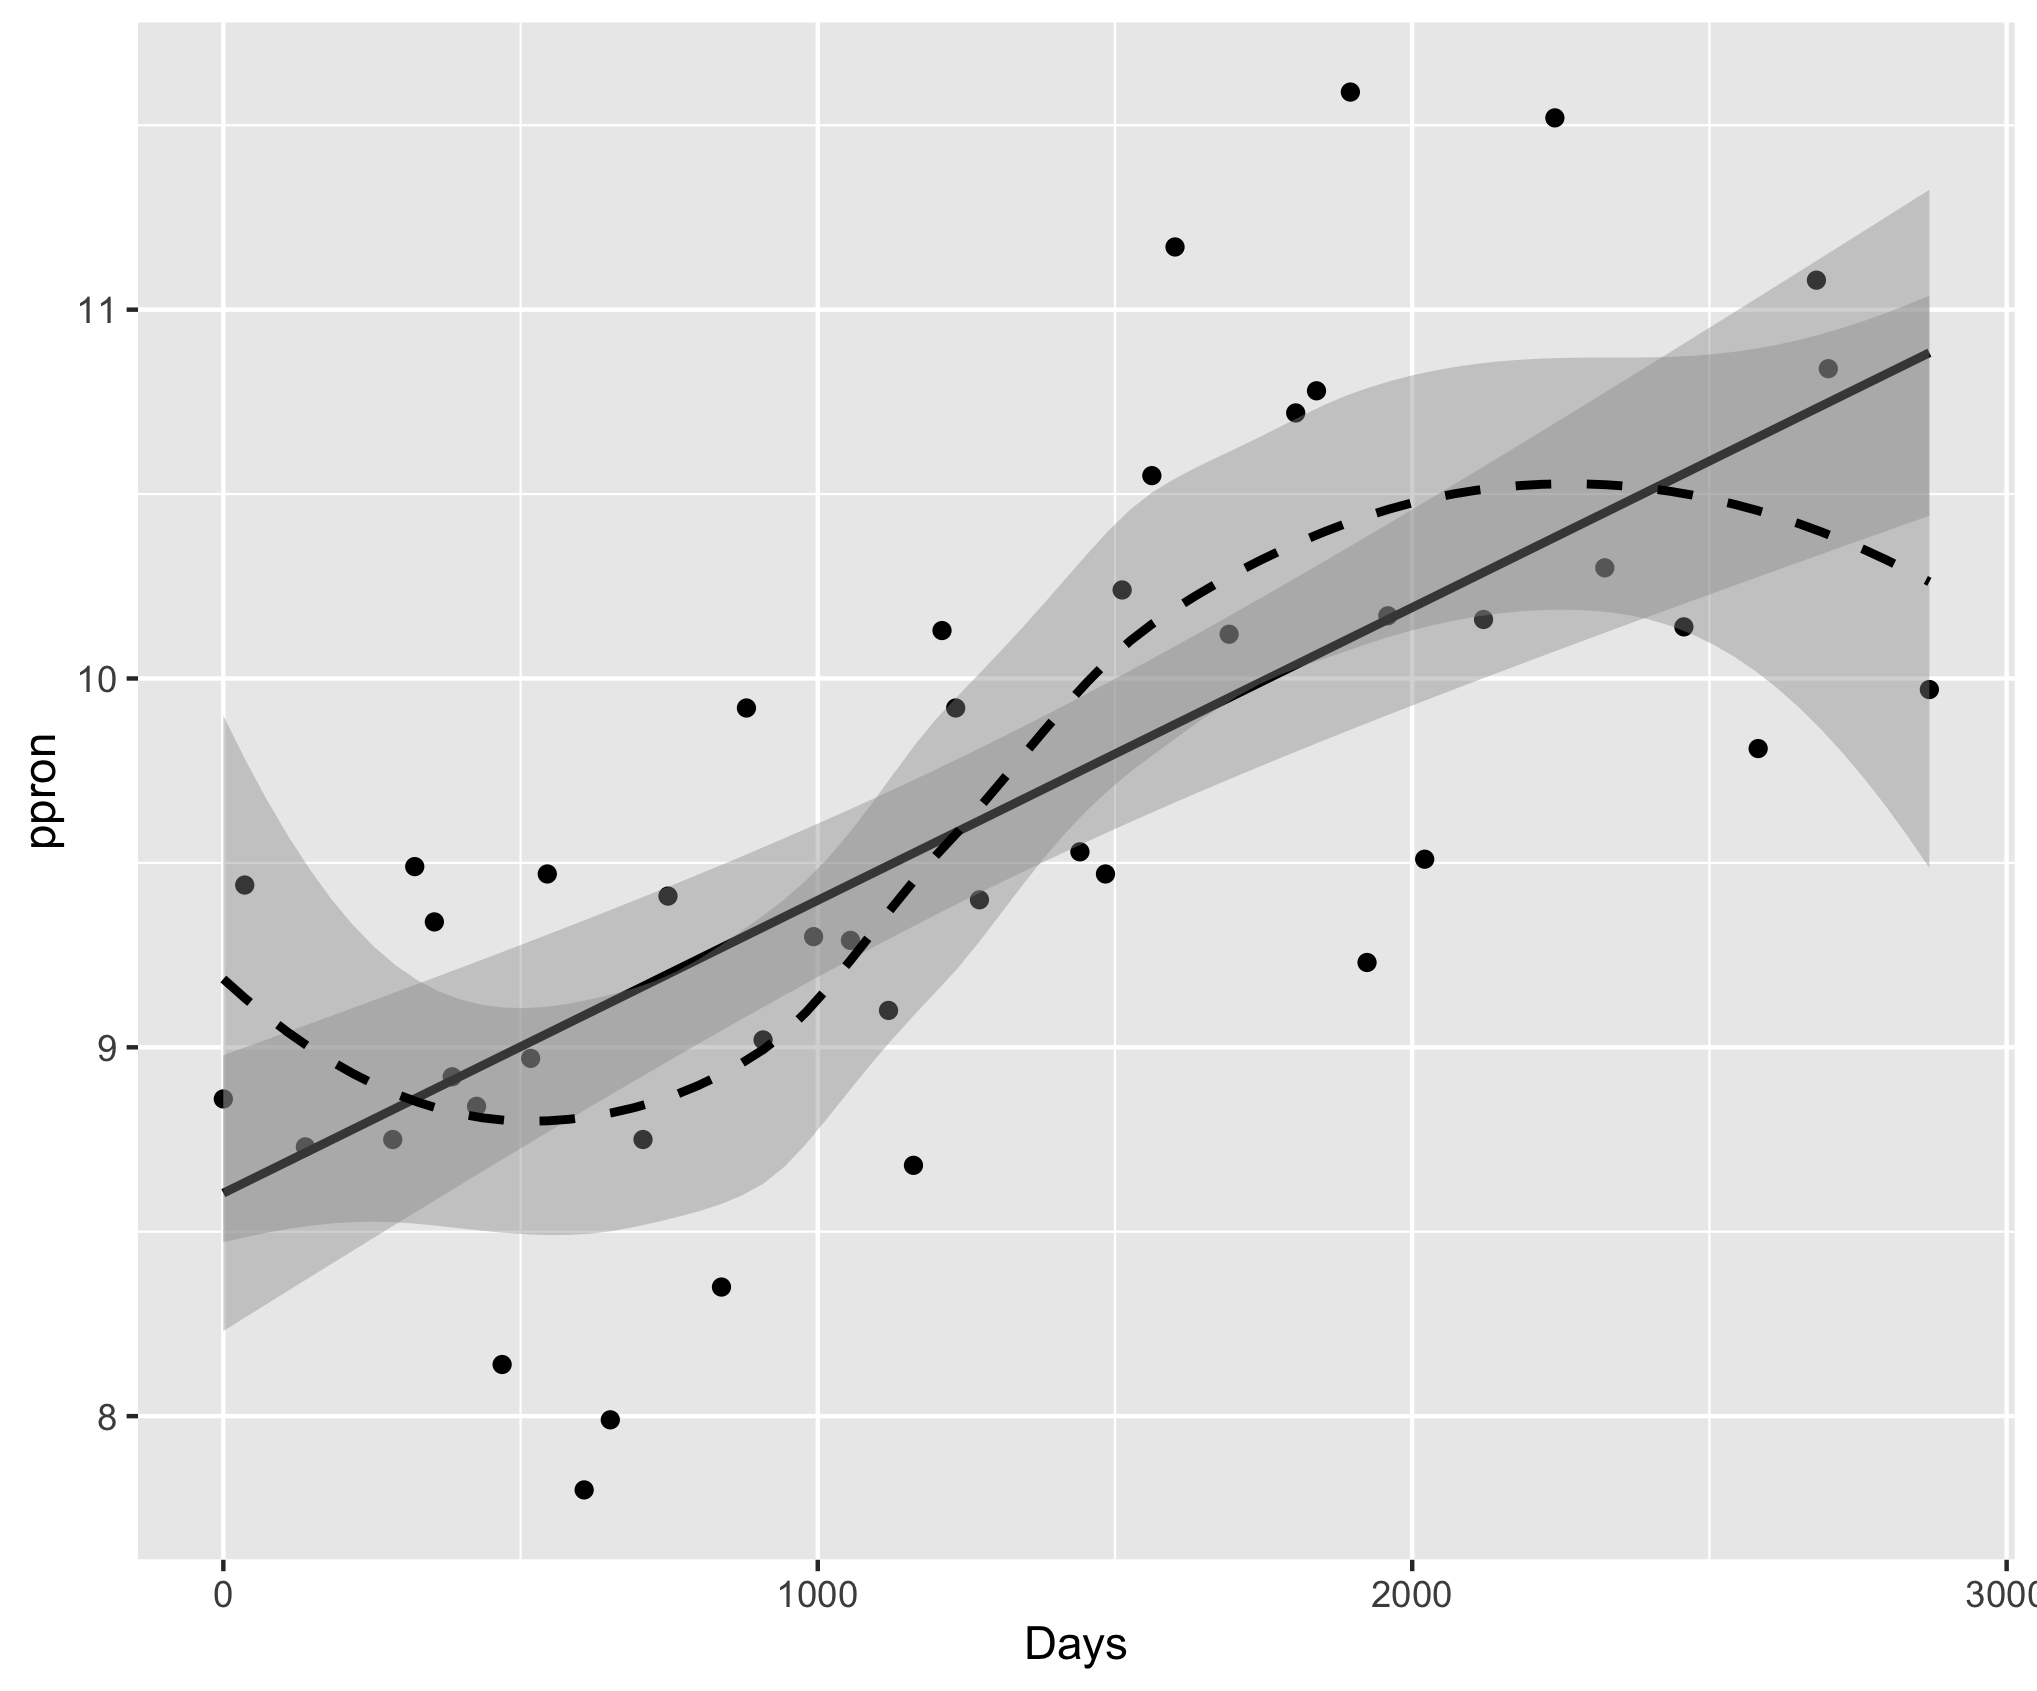
\includegraphics[width=6cm, height=5cm]{plots/comparison1.png}
	\caption{Comparing linear model with a non-linear model}
\end{figure}


This study extends the work of Berisha and Liss in a number of ways. Our hypotheses are:
\begin{enumerate}
	\item Language use of RR will be significantly different to our controls (GHWB, DJT).
	\item Modelling the dynamics of lexical features over time can be improved using non-linear models compared to linear models.
\end{enumerate}

\section{Methodology}\label{methodology}
We took the transcripts of 46 press conferences given by RR (from 1981 to 1988) and compared them with 134 press conferences (from 1989 to 1993) given by GHWB and 29 press conferences (from 2016 to 2019) conducted by DJT.  We analysed transcripts for language features (described below) shown to change longitudinally with AD. These language features are analysed at the word level, sentence level and document level. 
\par 
In the original study, GHWB was selected as the comparator president as he was the closest match in terms of age to RR (GHWB - age at the start of presidency: 64 years and 222 days vs RR: 69 years and 349 days). However, since his inauguration, DJT is now the closest comparible president in terms of age (DJT - age at the start of presidency: 70 years and 220 days). We included DJT who like GHWB has no known diagnosis of AD to determine whether the comparisons made by Berisha and Liss hold true with this closer presidential match in terms of age. 
\par 
We used the press conference transcripts in the American Presidency Project (APP) archive as a data source for this project. The APP is a comprehensive and organized searchable database of presidential documents, including transcripts of speeches, transcripts of news conferences, and other public documents. These documents are open access and can be downloaded at any time from the APP archive.

\subsection{Pre-processing}
To generate the files necessary for analysis, we downloaded each transcript and pre-processed each transcript in the following way. We omitted the prepared statement by the president and any speech by other individuals and started each transcript at the beginning of the first answer to a question by a member of the press. We filtered any annotations that were added to the transcript, including any references or clarifications, and any laughter. It is worth noting that there appears to be a difference in how 'hesitations' were marked down between each president. For RR \& DJT hesitations were marked by a single hyphen whereas for GHWB hesitations are marked by a double hyphen. In order to maintain consistency when parsing through the documents we changed both types of hesitation to be marked by a single hyphen. We also omitted one word answers to questions as this data would, from a theoretical perspective, not be relevant for language analysis. We did not make any alterations to the length of the document, but instead generated features which would normalise by the length of the document. We were therefore able to include all press conferences by the presidents analysed where there was a question and answer session conducted at least in part by the president (2 press conferences of GHWB were omitted due to a lack of a question and answer session).

\subsection{Feature Generation}
% We selected the type of processing as
Features were generated by running each transcript through a number of natural language processing libraries. We used the Natural Language ToolKit (NLTK) package \cite{Bird2009} in Python to stem each transcript using the Snowball Stemmer and also completed a part of speech (POS) tagging process. We also ran each transcript through Linguistic Inquiry and Word Count (LIWC) \cite{Pennebaker2015} software. We completed all NLP tasks in Python and completed all statistical analysis in R.. 
\par 
\subsubsection{Measures of lexical diversity}
Lexical diversity is a measure of the variety of language used within a given document and this is commonly used in the literature to measure language declinein those with MCI and AD \cite{Bucks2000, Le2012}. A document is said to have high lexical diversity if the number of unique words is large. We constructed four features of lexical variation. Firstly we looked at the number of unique words. To do this we split each transcript into individual words and changed them to lowercase using the NLTK package and were then count the number of unique words that appeared in each transcript. We also used the TTR formula, Brunet's Index and Honore's Statistic as other measures of lexical diversity \cite{Bucks2000}. For the formula's below, we use the following notation. N = total number of words, V = number of unique words and V1 = the number of words spoken exactly once.
\par 
Type token ratio (TTR) is the ratio obtained by dividing the types (The total number of different words) by the tokens (the total number of words in an utterance).
\begin{equation} \label{x1}
TTR = V / N
\end{equation}
\par 
Brunet's Index (W) differentiates itself from TTR, as it is not impacted by the length of the text itself. Brunet's Index is defined by the following equation:
\begin{equation} \label{x2}
W = N^{-0.165V}
\end{equation}
 Brunet's Index usually has a score of between 10 and 20, with high numbers indicating a more rich vocabulary compared to low numbers. \newline
\par 
Honore's Statistic is based on the idea that vocabulary richness is implied when a speaker uses a greater amount of unique words. This is indicated by the following equation: 
\begin{equation} \label{x3}
R = (100 \log N) / (1 - V1/V)
\end{equation}
\subsubsection{Fillers, Non-Specific Nouns and Low Imageability Verbs}
Fillers, Non-Specific Nouns and Low Imageability Verbs were features used by Berisha and Liss in their research \cite{Berisha2015} and were taken from work done by Bird et al \cite{Bird2000}. Fillers can be described as a potentially meaningless word that marks a pause or hesitation in speech. In those with MCI and AD, these words can be used to temporarily disguise problems in thought processes or word finding difficulties. Non-Specific Nouns refer to a category or an unspecified member of a given category, once again this can be characterised as a compensatory strategy for word finding difficulties. Imageability is characterized, according to Berisha and Liss\cite{Berisha2015}, as the ease with which a word provokes a mental image of what the word describes. 

\begin{table}[H]
	\begin{center}
	\begin{tabular}{ | p{3cm} | p{10cm} |}
		\hline
		Category & Words \\ \hline
		Fillers & \textit{"um", "uh", "er", "ah", "like", "okay", "right",  "you know", "well", "so", "basically", "actually", "literally"} \\ \hline
		Non Specific Nouns & \textit{"something", "anything", "thing", "everything"} \\ \hline
		LI Verbs & \textit{"be", "come", "do", "get", "give", go", "know", "look", "make", "see", "tell", "think", "want"} \\ \hline
	\end{tabular}
	\caption{\label{tab:table-name}Examples of words belonging to the categories Fillers, Non-Specific Nouns and Low Imageability Verbs}
	\end{center} 
\end{table}

\subsubsection{Usage of parts of speech}
Using a Part of Speech tagger (PoS) on each transcript analyses each sentence within the transcript and assigns a 'tag' to each word based on the function the word has in a sentence. At a basic level this can be divided into the eight defined parts of speech: 'nouns', 'pronouns', verbs', 'adjectives', 'adverbs', 'conjunctions', 'prepositions' and 'interjections' but can be further subcategorised. We used the PoS tagger built into NLTK to tag each transcript in turn and used the counts from each of these eight categories in our analysis. In addition to frequency counts we also normalised these features by dividing the frequency count by the number of words in the document to take into account transcript length.

\subsubsection{Linguistic Inquiry and Word Count(LIWC)}
The LIWC is a text processor / semantic tagger which analysis words within a given a document and compares the words in the LIWC dictionary file. The LIWC dictionary file contains over 6000 words which are categorised into approximately 90 different types. For example the word 'cried' is part of five word categories: sadness, negative emotion, overall affect, verbs and past focus \cite{Pennebaker2015}. Each word in the document or set of documents is searched for in the dictionary file and if found, the appropriate types is incremented by 1. What is output is an analysis of word usage in reference to each category. This is particularly useful in analysing both structural language changes but also the content or themes of language for a given transcript or set of transcripts.

\subsection{Longitudinal Analysis}
As with Berisha and Liss\cite{Berisha2015}, we analysed the transcripts over time in order to determine if there was an underlying temporal trend that may indicate that different parts of language increase or decrease over time. In AD, cognitive abilities are said to deteriorate over time and therefore it may be useful to analyse temporal trends that indicate a potential deterioration of cognition. In order to get a accurate measure of deterioration over time, we time stamped each transcript in relation to number of days from the first transcript to the date of the transcript being analysed as the press conferences were not evenly spaced out during the presidencies.
\par
We looked also compared the results of linear models and a non linear model in terms of best fit. The non linear model we used was the generalised additive model \cite{Hastie1986}.
There is evidence to support the idea that language deterioration. In figure 1, we look at the difference of between a linear model of Reagan's use of personal pronouns vs a non linear model. Whilst they are broadly similar in that they track an increase in his use of personal pronouns, they do not capture the variation in this increase as closely as a non linear model might. We therefore decided to apply this to all the features we extracted.

\section{Results}\label{results}
Two of the most important things to note are the wide variety of samples between the three presidents and also the varying timescales. RR participated in 46 press conferences over eight years (an average of 5.75 a year) which is the fewest number of press conferences given by an American president during their term of office. GHWB participated in 136 press conferences over four years (an average of 34 a year) and DJT participated in 29 press conferences to date (an average of 19.3 per year). 

\begin{table}[H]
	\begin{center}
	\begin{tabular}{ | p{3cm} | p{1.5cm} | p{1.5cm} | p{1.5cm} |}
		\hline
		& RR & GHWB & DJT \\ \hline
		Sample Size & 46 & 136 & 29 \\ \hline
		Total Words & 3423.91 (416.42) & 2607.72 (1210.38) & 1848.65 (1549.38) \\ \hline
		Unique Words & 894.13 (85.15) & 667.76 (218.67) & 481.82 (221.29) \\ \hline
		Mean Length of Utterance & 23.17 (1.402) & 18.71 (2.067) & 13.84 (1.619) \\ \hline
	\end{tabular}
	\caption{\label{tab:table-name}Means and Standard Deviations of general features for each set of transcripts}
	\end{center} 
\end{table}

In terms of more specific language differences between the presidents, as we found that RR used significantly more unique words, non-specific nouns and low imageability verbs than GHWB and DJT (see Table 3). The mean length of utterance for RR was significantly greater than that of GHWB and DJT. Some of these differences are due to the length of the sample, particularly in the case of DJT where his average sample is almost half the sample of RR. It could also be said that this could be due to differences in linguistic abilities or speaking style \cite{Berisha2015, Le2011}. However, we can certainly see that as controls GWHB and DJT are comparative in relation to non-specific nouns and LI verbs. 

\begin{table}[H]
	\begin{center}
	\begin{tabular}{ | p{3cm} | p{2.2cm} | p{2.2cm} | p{2.2cm} |}
		\hline
		& RR v GHWB & RR v DJT & GHWB v DJT \\ \hline
		Total Words & 6.6751 (574.8808, 1057.5324) & 5.352 (974.6629, 2175.8489) & 2.4774 (137.5811, 1380.5176) \\ \hline
		Unique Stems & 10.878 (161.1580, 232.6168) & 10.11 (275.4688, 414.0975) & 4.148 (75.86722, 219.92432) \\ \hline
		Mean Length of Utterance & 16.175 (3.915869, 5.009114) & 25.084 (8.453404, 9.922328)  & 13.484 (4.021601, 5.429148) \\ \hline	
		Non Specific Nouns & 9.2052 (5.881447, 9.13725) & 3.8627 (3.275567, 10.474625) & -0.37956 (-4.037218, 2.770237) \\ \hline
		LI Verbs & 4.0434 (10.84689, 31.53291) & 2.804 (10.91107, 67.41231) & 1.2836 (-11.06486, 49.00844)\\ \hline
	\end{tabular}
	\caption{\label{tab:table-name}RR T-tests vs GWB and DJT, T-statistic and 95\%confidence intervals}
	\end{center} 
\end{table}

\subsection{Longitudinal Analysis}
\subsubsection{Comparison of Ronald Reagan and George H.W. Bush}
We then looked at the data from a longitudinal perspective as we were interested in seeing whether we can track various language features and their progress over time. We ran a number of Pearsons correlations with number of days as a time reference (we calculated this as the total number of days from the first sample) and the dependent variables. We also calculated these Pearsons correlations with transcript index number as a time reference and the dependant variables as a replication of the Berisha and LIss study \cite{Berisha2015} and these results are described in the supplementary material.


For our controls, we found them to be stable for the most part with the main highlights being a decrease in Adverb usage for DJT (R=-0.36, p=0.049) and a steady but not severe decline in a number of variables for GWHB, namely total word count, unique words, low imageability words and verb usage.
\par 
For RR, his decline is more marked and more widespread through his language use. We noticed an significant increase in adverb (R=0.41, p=0.004) and pronoun usage (R=0.65, p\textless0.001), as well as a slight usage increase in Non-specific nouns(R=0.30, p=0.03). There was also a significant decrease in number of unique words (R=-0.56, p\textless0.001) and noun usage (R=-0.70, p\textless0.001). Also there was a significant decrease in adjective usage (R=-0.40, p=0.005) and a significant decrease in total word count (R=-0.31, p=0.03). 
\par
Given the number of hypotheses being tested, we felt it was necessary to control for false discovery rate and therefore Benjamii-Yekutieli procedure was applied to the results of the analysis. By applying this, we produced a final list of important features for each president. For RR, this was 22 features and for GHWB this was 14 features.  The features were generated from multiple sources and therefore there was some significant overlap between the features but for completeness we have included all features in Table 6. 

\begin{table}[H]
	\begin{center}
	\begin{tabular}{ | l | c | c |}
		\hline
		& RR R-Squared  & GWB R-Squared \\ \hline
		ppron & \textbf{0.700***} & 0.007 \\ \hline
		social & \textbf{0.698***} & 0.204 \\ \hline
		NounsNormalised & \textbf{-0.689***} & -0.023 \\ \hline
		function & \textbf{0.670***} & -0.169 \\ \hline
		conj &\textbf{0.644***} & -0.452 \\ \hline
		PronounsNormalised & \textbf{0.631***} & 0.131 \\ \hline
		Analytic & \textbf{-0.626***} & -0.013 \\ \hline
		NN & \textbf{-0.601***} & -0.197 \\ \hline
		male & \textbf{0.585***} & 0.024 \\ \hline
		UniqueWords & \textbf{-0.578***} & -0.257 \\ \hline
		WDT & \textbf{-0.577***} & -0.173 \\ \hline
		shehe & \textbf{0.529*} & -0.005 \\ \hline
		VBZ & \textbf{-0.521*} & -0.157 \\ \hline
		JJ & \textbf{-0.518*} & -0.206 \\ \hline
		Fillers & -0.076 & \textbf{-0.359**} \\ \hline	
		EX & -0.193* & \textbf{-0.337**} \\ \hline	
		achieve & -0.248 & \textbf{0.334**} \\ \hline		
		\multicolumn{3}{@{}p{1.5in}}{\footnotesize * denotes p\textless 0.05} \\
    	\multicolumn{3}{@{}p{1.5in}}{\footnotesize ** denotes p\textless 0.01} \\
    	\multicolumn{3}{@{}p{1.5in}}{\footnotesize *** denotes p\textless 0.001} \\
	\end{tabular}
	\caption{\label{tab:table-name}Pearson Correlations for Features}
	\end{center} 
\end{table}

\subsubsection{Comparison of Ronald Reagan and Donald J. Trump}
\begin{table}[H]
	\begin{center}
	\begin{tabular}{ | l | c | c |}
		\hline
		& RR R-Squared & DJT R-Squared \\ \hline
		ppron & \textbf{0.700***} & 0.007 \\ \hline
		social & \textbf{0.698***} & 0.204 \\ \hline
		NounsNormalised & \textbf{-0.689***} & -0.023 \\ \hline
		function & \textbf{0.670***} & -0.169 \\ \hline
		conj &\textbf{0.644***} & -0.452 \\ \hline
		PronounsNormalised & \textbf{0.631***} & 0.131 \\ \hline
		Analytic & \textbf{-0.626***} & -0.013 \\ \hline
		NN & \textbf{-0.601***} & -0.197 \\ \hline
		male & \textbf{0.585***} & 0.024 \\ \hline
		UniqueWords & \textbf{-0.578***} & -0.257 \\ \hline
		WDT & \textbf{-0.577***} & -0.173 \\ \hline
		shehe & \textbf{0.529*} & -0.005 \\ \hline
		VBZ & \textbf{-0.521*} & -0.157 \\ \hline
		JJ & \textbf{-0.518*} & -0.206 \\ \hline
		Fillers & -0.076 & \textbf{-0.359**} \\ \hline	
		EX & -0.193* & \textbf{-0.337**} \\ \hline	
		achieve & -0.248 & \textbf{0.334**} \\ \hline		
		\multicolumn{3}{@{}p{1.5in}}{\footnotesize * denotes p\textless 0.05} \\
    	\multicolumn{3}{@{}p{1.5in}}{\footnotesize ** denotes p\textless 0.01} \\
    	\multicolumn{3}{@{}p{1.5in}}{\footnotesize *** denotes p\textless 0.001} \\
	\end{tabular}
	\caption{\label{tab:table-name}Pearson Correlations for Features}
	\end{center} 
\end{table}
% Needs explanation

\subsection{Comparing linear models and non-linear models}
In terms of comparing the general additive model and linear models. We calculated the predicted residual error sum of squares (PRESS) statistic for each feature is a form of cross-validation used in regression analysis to provide a summary measure of the fit of a model to a sample of observations that were not themselves used to estimate the model. There were no significant differences (paired t-test: t=1.8875, df  = 21, p-value = 0.07299). 

\begin{table}[H]
	\begin{center}
	\begin{tabular}{ | l | c | c |}
		\hline
		Feature & GAM Press Statistic & LM Press Statistic \\ \hline
		ppron & 18.591104613 & 20.001055542 \\ \hline
		social & 21.681732112 & 24.906646115  \\ \hline
		NounsNormalised & 0.002818941 & 0.002797798\\ \hline
		function & 46.546071705 & 46.031993602 \\ \hline
		conj & 8.812330188 & 8.354974826 \\ \hline
		PronounsNormalised & 0.002284437 & 0.002356129\\ \hline
		Analytic & 2272.200519272 & 2239.224863610 \\ \hline
		Pronoun & 44.557282749 & 46.894576916 \\ \hline		
		NN & 101685.870974277 & 96485.575598505 \\ \hline
		male & 5.191815443 & 5.278559152 \\ \hline
		UniqueWords & 255114.636660673 & 238042.427437454 \\ \hline
		WDT & 1987.149134694 & 1958.781236655 \\ \hline
		nouns & 276723.222762842 & 262192.120091097 \\ \hline
		nouns/100 & 27.670762078 & 26.219212009 \\ \hline
		UniqueStems & 170450.645283172 & 166302.725530118 \\ \hline
		shehe & 5.188136314 & 5.265385185 \\ \hline
		VBZ & 13889.871831536 & 13721.175422577 \\ \hline
		JJ & 24950.440222526 & 24692.043386181 \\ \hline
		article & 13.500676675 & 13.468083961 \\ \hline	
		Adjectives & 30210.006270270 & 29865.240707991 \\ \hline	
		Adjectives.100 & 3.020898615 & 2.986524071 \\ \hline
		Dic & 40.099289973 & 38.501060715 \\ \hline	
	\end{tabular}
	\caption{\label{tab:table-name}Comparison of GAM and Linear Model using the PRESS statistic}
	\end{center} 
\end{table}

\section{Discussion}\label{discussion}
President Reagan received his diagnosis of AD in August 1994 but using transcripts of speeches he made in his two terms as President (January 1981 - January 1989) we have been able to identify a number of changes in his use of language that we might ascribe to the onset of MCI and early AD. Despite differences in our methodology, our research supports some of the findings of Berisha and Liss in that we find an increase in non-specifc noun usage. Compared to our controls (GWHB and DJT), we find some slight trends with GWHB but no such trends with DJT in his speech albeit his samples of speech span a shorter period of time. Interestingly, when we normalised the various types of words used by the presidents we found some interesting patterns that further differentiated RR from the controls. Whilst Non-specific nouns increased over time, we found that noun usage in general significantly decreased and pronouns increased similarly significantly. The increase in pronoun for those with early AD has been identified in literature, although there are only a few studies that explore this \cite{Wendelstein2015}. Wendlestein et al propose that the increased used of pronouns is an expression of an impaired ability to adapt language to the listener's needs \cite{Wendelstein2015}. Almor et al attributed this reliance on pronouns due to an impaired working memory \cite{Almor1999}.
\par 
The decrease in overall noun usage has also been identified as a feature. Jarrold et al found that AD patients would use more pronouns, more verbs and fewer nouns than controls \cite{Jarrold2014}. Wendlestein in their investigations into noun usage found that noun usage decreased later on in AD progression and was unaffected in the pre-clinical stages of AD \cite{Wendelstein2014}. Our results are supported by existing literature and this potentially means that language analysis in the way we have structured it may have diagnostic or prognostic properties.
\par 
A criticism of Berisha and Liss's work is the problems they had with normalising the transcripts in terms of length. This was also a problem in the work of Garrard et al \cite{Garrard2005, Le2011}. Whilst it is important to control for outliers, there are other ways in which we can control for length of sample. In this paper, we controlled for transcript length by dividing any features that were raw counts by the total length of the transcript. When we did this, we found that there was a significant decrease in the number of unique words (R=-0.56, p\textless0.001) used. However when we controlled via normalisation as described above, we found that this was not a significant feature (R=-0.172, p=0.25). 
\par 
Overall, we are able to show differences in the a number of language features between RR, GHWB and DJT over time and the psychological literature confirms our findings with reference to these changes.
\par
Our next hypothesis involved exploring whether linear models were the most appropriate way to track this longitudinal data. In our analysis, we found there was no significant difference in terms of mean sum of squares errors between the linear model and the generalised additive model. However this does not mean that these are equivalent. For example, consider Figure 2. We compare a model fit to a linear model with a generalised additive model which aims to model the data more closely. It is clear to see that both models can track the movements of language use over time however, the linear model is quite a rigid model which does not allow for different inflection points. We can see that RR's decline is not linear, and that there are periods of relative stability and some periods where the decline is more severe. We argue that these more nuanced changes over time can only be modelled by a model such as a GAM.
\par
In her paper on developing diagnositic criteria for Mild Cognitive Impairment, Albert et all \cite{Albert2011} states 'it is important to obtain longitudinal assessments of cognition, whenever possible' and 'obtaining objective evidence of progressive declines in cognition over time is important for establishing the accuracy of the diagnosis, as well as for
assessing any potential treatment response.' As we have shown, it is not the case that language declines in a linear way and whilst we have a number of data points that we can use to model RR's decline, in a clinical setting it would be impractical to have upwards of 40 data collection points. We feel that  it is important that we have more than just two. In the figure 2 and figure 3 below, we can see that if we measured language at Reagan's first transcript to a point after 700 days the vast majority of points would point to a decline in language. However, the next figure shows what would happen if we measured language from Reagan's second transcript, just 34 days later. In this case, we can see that in some cases we would mark Reagan as improving when it is clear that he is not.

\begin{figure}[H]
	\centering
	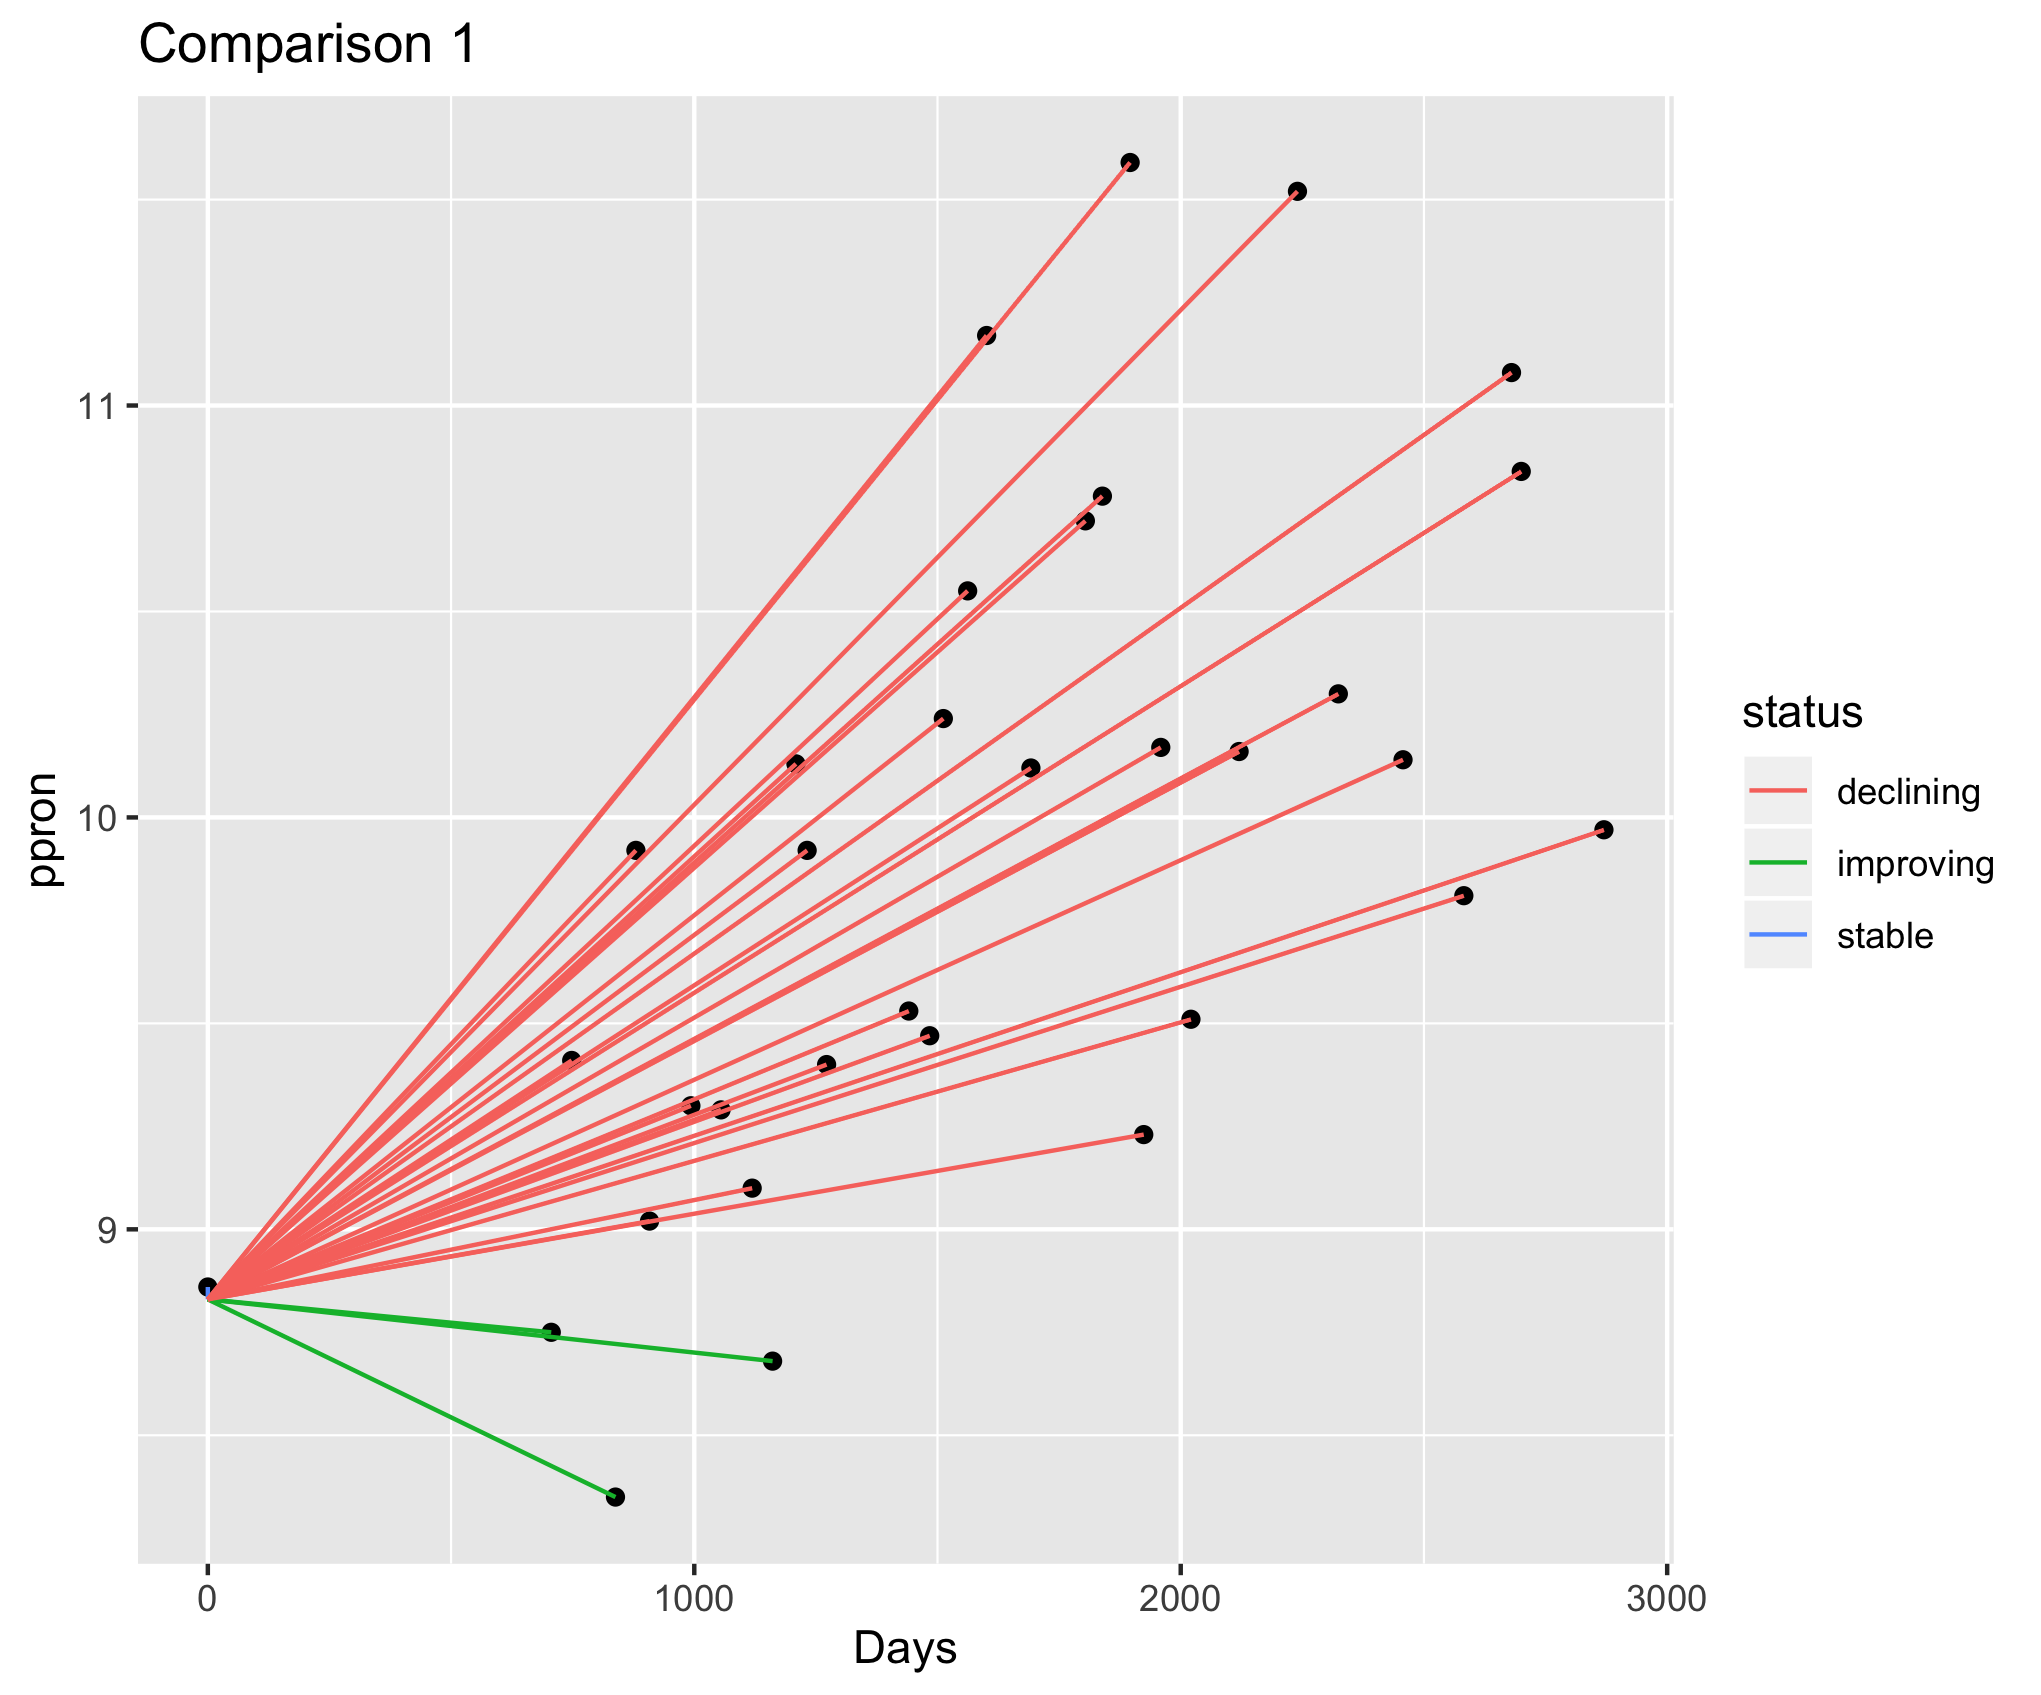
\includegraphics[width=6cm, height=5cm]{plots/comp1.png}
	\caption{Measuring decline from Reagan's first transcript to all other transcripts greater than 700 days later}
\end{figure}

\begin{figure}[H]
	\centering
	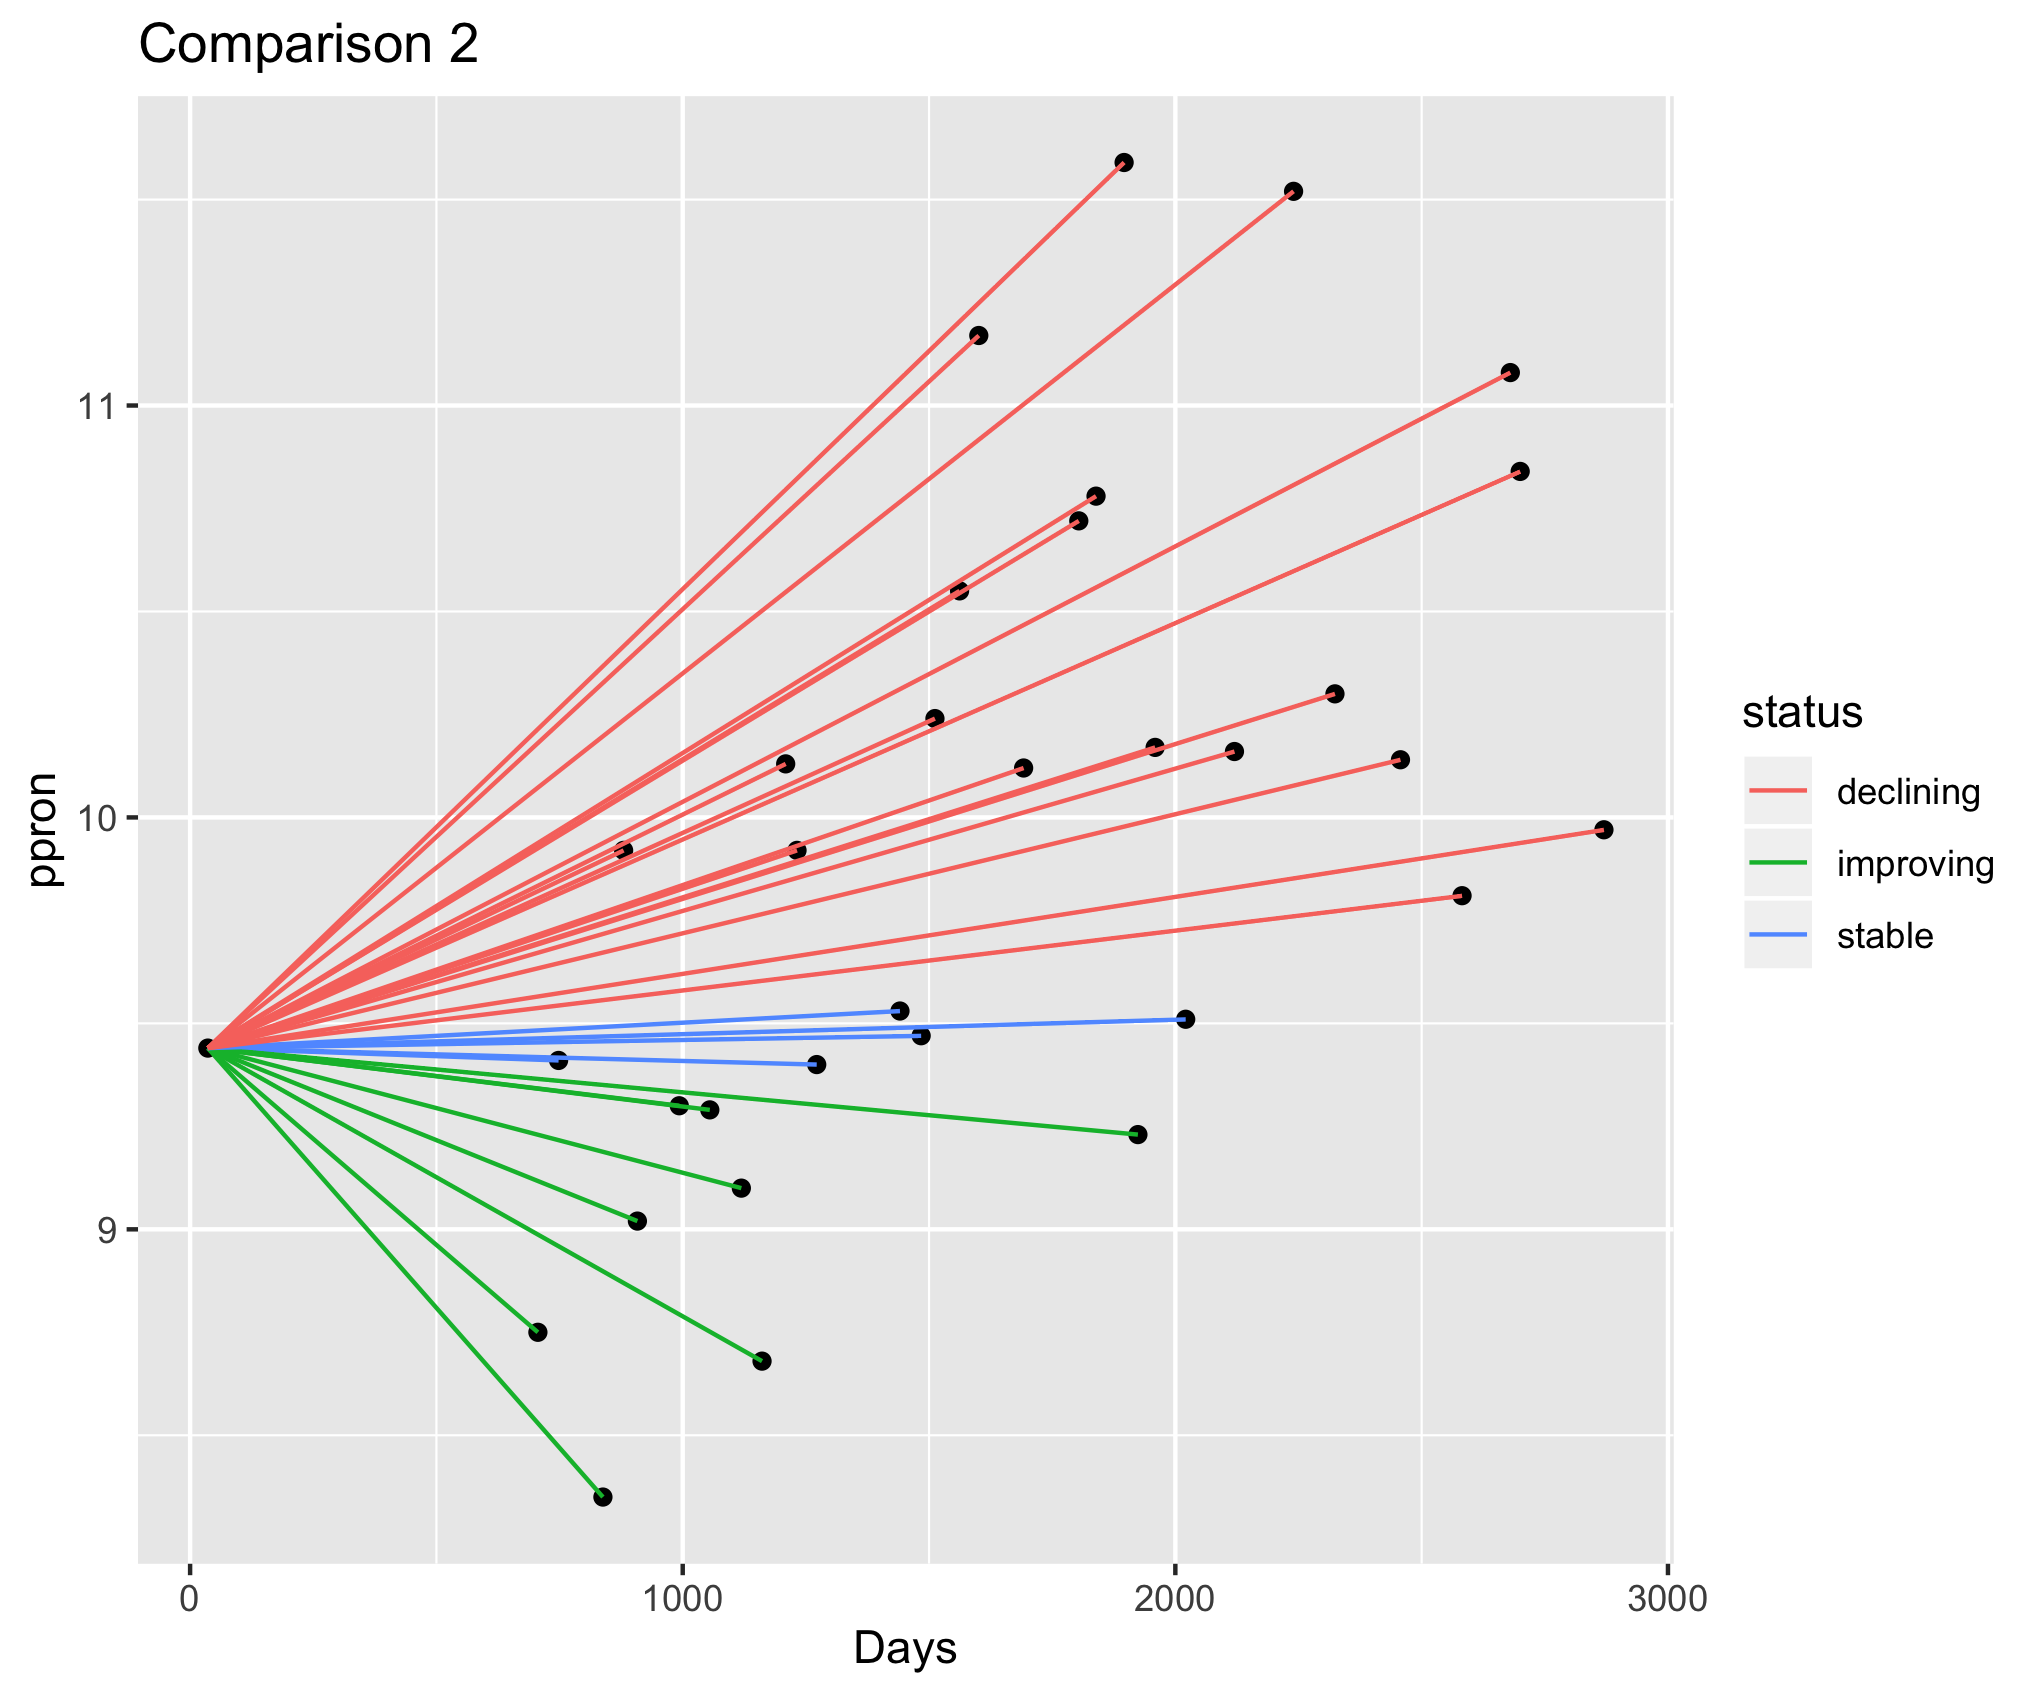
\includegraphics[width=6cm, height=5cm]{plots/comp2.png}
	\caption{Measuring decline from Reagan's first transcript to all other transcripts greater than 700 days later}
\end{figure}
\par 
There are limitations of this research. Whilst in terms of age, DJT is certainly more suitable as a control to match with RR, in some ways they held very different styles of press conferences in that RR preferred to do solo press conferences and DJT has shown a preference for doing joint press conferences which have an impact on the amount of language produced. This artefact of the data is in itself notable as it illustrates the problems we may have with smaller amounts of speech and the problem of finding an appropriate control is a common one in this domain, given the considerable variation in factors such as age, language ability and education. As mentioned above, we are lucky enough to have numerous samples of data collected over a long period of time and this is not something that can be easily translated to a clinical protocol. Finally, the variability in the number and quality of the transcriptions raises some doubts as to the results of DJT. Is it the lack of instances of data, or that the number of words per transcript is significantly less than with RR or GHWB. This does have further implications for using a protocol such as this in a more general way as it will impact how data is collected. 
\par 
With further work, it is not feasible to have a vast array of samples over a timeframe, as we have had with the president corpus and so it would be worth exploring how the quality of these predictions may lessen when faced with considerably fewer samples and over a smaller time period. It would also be worth extending this research further to encompass more of the linguistic features Fraser used in her work \cite{Fraser2015} to see if there are any further insights to be gained. In addition, this replication and extension has demonstrated the potential utility of using longitudinal data as a means of comparing language use of a person at two or more time periods and using this information as a diagnostic aid for MCI and therefore more work would be helpful from a longitudinal perspective to see if this approach may be valid in moving towards a solution for this particular problem. 

\section{Conclusions}\label{conclusions}
The results of this work show that we can track a person's use of language through time in a number of ways and that it is possible for an individual to be his or her own control. This is important as it means the heterogenous nature of the MCI population does not impact results as much as if we were comparing those with group of MCI patients with a group of controls. Equally, it would be helpful to have controls to ascertain what would be usual to expect in the decline of language in a healthy older adult. 
\par 
The results of this work also identify some clues as to what could work in a clinical setting, or how we might be able to collect data in a way that accurately tracks language decline without making incorrect assumptions. 
\par
From a clinical perspective, we can see that using samples (albeit for this dataset) is able to track languages changes over a given time frame. This potentially means that we can use a similar methodology to collect regular language samples in settings such as memory clinics and GP's surgeries and even potentially in the people's homes and that these language samples, have the potential to act as an early warning sign for Mild Cognitive Impairment that potentially will identify patients at risk of developing Alzheimer's Disease.
\bibliographystyle{ieeetr}
\bibliography{main}

%\begin{table}[H]
%	\begin{center}
%	\begin{tabular}{ | l | p{1.5cm} | p{1.5cm} | p{1.5cm} |}
%		\hline
%		& RR & GHWB & DJT \\ \hline
%		Word Count & \textbf{-0.31*} & \textbf{-0.21*} & 0.08 \\ \hline 
%		Unique Words & \textbf{-0.56***} & \textbf{-0.25**} & 0.16 \\ \hline
%		Non Specific Nouns & \textbf{0.30*} & -0.08 & -0.03 \\ \hline
%		LI Verbs & -0.19 & \textbf{-0.20**} & 0.02 \\ \hline
%		Nouns Normalised & \textbf{-0.70***} & -0.03 & 0.14 \\ \hline
%		Verbs Normalised & \textbf{0.36**} & \textbf{0.24***} & -0.03 \\ \hline
%		Adjectives Normalised & \textbf{-0.40**} & 0.08 & -0.34 \\ \hline
%		Adverbs Normalised & \textbf{0.41***} & 0.02 & \textbf{-0.36*} \\ \hline
%		Pronouns Normalised & \textbf{0.65***} & 0.13 & 0.07 \\ \hline
%		\multicolumn{4}{@{}p{1.5in}}{\footnotesize * denotes p\textless 0.05} \\
%    	\multicolumn{4}{@{}p{1.5in}}{\footnotesize ** denotes p\textless 0.01} \\
%    	\multicolumn{4}{@{}p{1.5in}}{\footnotesize *** denotes p\textless 0.001} \\
%	\end{tabular}
%	\caption{\label{tab:table-name}Pearson Correlations for Features}
%	\end{center} 
%\end{table}

\end{document}
